%==============================================================
%  EE201 -- Circuit Theory I
%  Lecture 1 : Basic Concepts
%  M. Mert Ankaralı, METU EEE
%
%  Compile:  ./build.sh      (or: pdflatex EE201_Lecture_1.tex, twice)
%==============================================================
\documentclass[11pt,a4paper]{article}

%-------------------- packages --------------------------------
\usepackage[T1]{fontenc}
\usepackage[utf8]{inputenc}
\usepackage[english]{babel}
\usepackage{lmodern}
\usepackage[margin=2.3cm,top=2.0cm,bottom=1.9cm,headheight=14pt,headsep=9pt]{geometry}
\usepackage{amsmath,amssymb}
\usepackage{array,booktabs,tabularx}
\usepackage{enumitem}
\usepackage[table]{xcolor}
\usepackage{fancyhdr}
\usepackage{titlesec}
\usepackage{graphicx}
\usepackage[most]{tcolorbox}
\usepackage{tikz}
\usepackage[american,siunitx]{circuitikz}
\usetikzlibrary{arrows.meta,positioning,calc,decorations.pathmorphing,decorations.pathreplacing,patterns,shapes.geometric}
\usepackage[colorlinks=true,allcolors=metured,breaklinks=true]{hyperref}

%-------------------- colour system ---------------------------
% One colour per physical quantity, used identically in the slides.
\definecolor{metured}{RGB}{155,27,48}    % headings, structure
\definecolor{metugray}{RGB}{88,89,91}
\definecolor{ccur}{RGB}{0,102,170}       % CURRENT  -- blue
\definecolor{cvolt}{RGB}{214,120,0}      % VOLTAGE  -- orange
\definecolor{cpow}{RGB}{23,128,74}       % POWER / ENERGY -- green
\definecolor{ccharge}{RGB}{124,60,160}   % CHARGE   -- purple
\definecolor{boxgray}{RGB}{245,245,245}

\newcommand{\Icol}[1]{\textcolor{ccur}{#1}}
\newcommand{\Vcol}[1]{\textcolor{cvolt}{#1}}
\newcommand{\Pcol}[1]{\textcolor{cpow}{#1}}
\newcommand{\Qcol}[1]{\textcolor{ccharge}{#1}}

%-------------------- units (no siunitx dependency) -----------
\newcommand{\uni}[1]{\,\mathrm{#1}}
\newcommand{\A}{\uni{A}}   \newcommand{\V}{\uni{V}}
\newcommand{\W}{\uni{W}}   \newcommand{\J}{\uni{J}}
\newcommand{\Cb}{\uni{C}}  \newcommand{\s}{\uni{s}}

%-------------------- layout ----------------------------------
\pagestyle{fancy}
\fancyhf{}
\lhead{\small\textcolor{metugray}{EE201 -- Circuit Theory I}}
\rhead{\small\textcolor{metugray}{Lecture 1: Basic Concepts}}
\cfoot{\small\thepage}
\renewcommand{\headrulewidth}{0.4pt}

\titleformat{\section}{\large\bfseries\color{metured}}{\thesection.}{0.6em}{}
\titleformat{\subsection}{\normalsize\bfseries\color{metugray}}{\thesubsection.}{0.6em}{}
\titlespacing*{\section}{0pt}{1.4ex plus .3ex}{0.7ex}
\titlespacing*{\subsection}{0pt}{1.1ex plus .2ex}{0.5ex}

\setlist[itemize]{itemsep=2pt,topsep=3pt,parsep=0pt,leftmargin=1.5em}
\setlist[enumerate]{itemsep=2pt,topsep=3pt,parsep=0pt,leftmargin=1.7em}
\setlength{\parindent}{0pt}
\setlength{\parskip}{0.7ex plus .1ex}
\raggedbottom
\widowpenalty=10000
\clubpenalty=10000
\brokenpenalty=10000

%-------------------- boxes -----------------------------------
\newtcolorbox{definitionbox}[1]{enhanced,
  colback=metured!4, colframe=metured, boxrule=0.9pt,
  fonttitle=\bfseries, title={#1}, arc=2pt,
  left=7pt,right=7pt,top=5pt,bottom=5pt, before skip=7pt, after skip=7pt}

\newtcolorbox{ideabox}[1][Key idea]{enhanced,
  colback=ccur!5, colframe=ccur, boxrule=0.9pt,
  fonttitle=\bfseries, title={#1}, arc=2pt,
  left=7pt,right=7pt,top=5pt,bottom=5pt, before skip=7pt, after skip=7pt}

\newtcolorbox{examplebox}[1][Example]{enhanced,
  colback=cpow!4, colframe=cpow, boxrule=0.9pt,
  fonttitle=\bfseries, title={#1}, arc=2pt,
  left=7pt,right=7pt,top=5pt,bottom=5pt, before skip=7pt, after skip=7pt}

\newtcolorbox{cautionbox}[1][Careful]{enhanced,
  colback=cvolt!6, colframe=cvolt, boxrule=0.9pt,
  fonttitle=\bfseries, title={#1}, arc=2pt,
  left=7pt,right=7pt,top=5pt,bottom=5pt, before skip=7pt, after skip=7pt}

%-------------------- circuitikz defaults ---------------------
\ctikzset{bipoles/length=0.9cm, color=black,
          label/align=straight}
\tikzset{
  curarr/.style={-{Stealth[length=2.6mm]}, ccur, very thick},
  volarr/.style={-{Stealth[length=2.6mm]}, cvolt, very thick},
  blk/.style={draw=metugray, fill=boxgray, rounded corners=2pt,
              minimum height=1.25cm, text width=2.9cm, align=center, font=\small},
  flowarr/.style={-{Stealth[length=3mm]}, metured, very thick},
}

%==============================================================
\begin{document}

%-------------------- title block -----------------------------
\begin{center}
\begin{tcolorbox}[enhanced, colback=metured!5, colframe=metured, boxrule=1pt,
                  arc=3pt, left=10pt,right=10pt,top=7pt,bottom=7pt, width=\textwidth]
\begin{center}
  {\small\scshape Middle East Technical University}\\[2pt]
  {\small\scshape Department of Electrical and Electronics Engineering}\\[7pt]
  {\Large\bfseries\color{metured} EE201 -- Circuit Theory I}\\[4pt]
  {\large\bfseries Lecture 1: Basic Concepts}\\[6pt]
  {\small M. Mert Ankaralı}
\end{center}
\end{tcolorbox}
\end{center}

\vspace{-0.5em}

%-------------------- how to use ------------------------------
\begin{center}
\small
\begin{tabular}{@{}l l@{}}
\toprule
\multicolumn{2}{@{}l}{\textbf{Colour code used in these notes and in the slides}}\\
\midrule
\Qcol{$\blacksquare$}~charge $q$ & \Icol{$\blacksquare$}~current $i$ \quad
\Vcol{$\blacksquare$}~voltage $v$ \quad \Pcol{$\blacksquare$}~power $p$, energy $w$\\
\bottomrule
\end{tabular}
\end{center}

%==============================================================
\section{Why circuits? From the world to a model}

Circuit theory is not about wires. It is a way of \emph{modelling} physical systems, and
you will use the same thinking in control, signal processing, power, robotics and
electronics for the rest of your career. The pipeline is always the same:

\begin{center}
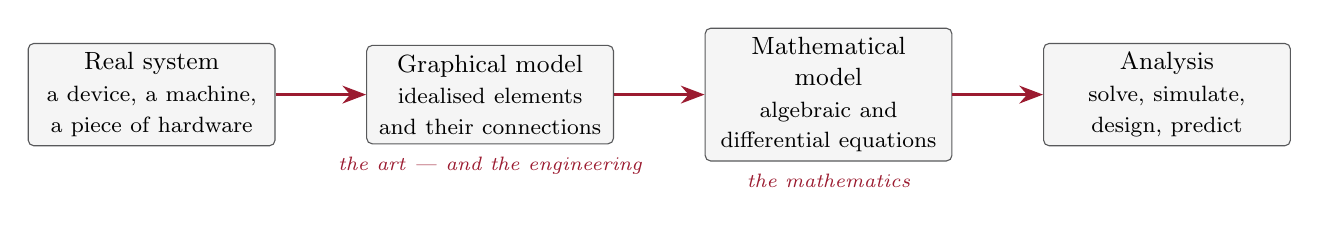
\begin{tikzpicture}[node distance=1.15cm]
  \node[blk] (a) {Real system\\[2pt] \footnotesize a device, a machine,\\ \footnotesize a piece of hardware};
  \node[blk, right=of a] (b) {Graphical model\\[2pt] \footnotesize idealised elements\\ \footnotesize and their connections};
  \node[blk, right=of b] (c) {Mathematical model\\[2pt] \footnotesize algebraic and\\ \footnotesize differential equations};
  \node[blk, right=of c] (d) {Analysis\\[2pt] \footnotesize solve, simulate,\\ \footnotesize design, predict};
  \draw[flowarr] (a) -- (b);
  \draw[flowarr] (b) -- (c);
  \draw[flowarr] (c) -- (d);
  \node[below=1pt of b, font=\scriptsize\itshape, text=metured] {the art --- and the engineering};
  \node[below=1pt of c, font=\scriptsize\itshape, text=metured] {the mathematics};
\end{tikzpicture}
\end{center}

The hard step is the first arrow. A real resistor has inductance, a temperature
coefficient, a power rating and a size; we throw all of that away and keep one number,
$R$. Whether that is brilliant or foolish depends on what you ask of the model. Calling
that step ``the art'' makes it sound decorative, as though the equations were the real
work. The opposite is true: the mathematics can be looked up, while deciding what to keep
and what to discard \emph{is} the engineering.

\begin{center}
\begin{minipage}{0.82\textwidth}
\centering
{\large\itshape ``All models are wrong, but some are useful.''}\\[3pt]
{\small\color{metugray} George E. P. Box, \emph{Science and Statistics}, 1976}
\end{minipage}
\end{center}

Every element you will meet in EE201 is wrong in some measurable way. The question is
never ``is this model true?'' but ``is it useful here?''.

\begin{center}
\begin{circuitikz}[scale=0.95, transform shape]
  \draw (0,0) to[battery1, invert, l_={$v_s$}] (0,2.6);
  \draw (0,2.6) to[R, l=$R_1$, i>^={\color{ccur}$i$}] (2.8,2.6) coordinate (x);
  \node[op amp, anchor=-, scale=0.95] (oa) at (2.8,2.6) {};
  \draw (oa.+) -- ++(-0.7,0) coordinate (gp) -- (gp |- 0,0);
  \draw (x) -- ++(0,1.5) coordinate (ft);
  \draw (ft) to[R, l=$R_f$] (ft -| oa.out) coordinate (fr);
  \draw (fr) -- (oa.out);
  \draw (oa.out) -- ++(0.45,0) coordinate (o1);
  \draw (o1) to[R, l=$R_2$] ++(2.4,0) coordinate (b);
  \draw (b) to[C, l_=$C$] (b |- 0,0);
  \draw (0,0) -- (b |- 0,0);
  \draw (1.4,0) node[ground]{};
  \fill[metured] (b) circle (2pt);
  \node[font=\small, text=cvolt, right=3pt] at (b) {$v_{\mathrm{out}}$};
\end{circuitikz}
\end{center}

\vspace{-0.3em}
{\small A circuit you will be able to analyse by the end of the semester: a source,
resistors, an operational amplifier and a capacitor --- one element from each part of the
course. All of EE201 is about what each element does on its own, and what the wires force
them to share.}

\begin{ideabox}[The same pipeline, other domains]
The elements change, the structure does not. Every such domain has one \emph{across}
quantity and one \emph{through} quantity:

\begin{center}
\small
\begin{tabular}{@{}l l l@{}}
\toprule
\textbf{Domain} & \textbf{``Across'' quantity} & \textbf{``Through'' quantity}\\
\midrule
electrical & electric potential & current\\
hydraulic  & pressure           & volumetric flow rate\\
thermal    & temperature        & heat flow\\
mechanical & velocity           & force\\
\bottomrule
\end{tabular}
\end{center}

An across quantity is always a \emph{difference} between two points, and in every domain
the word ``difference'' is dropped. Sometimes for convenience: ``the voltage across
$R_2$'' names no terminals, yet nobody is confused. More often because a \emph{reference}
was agreed on long ago --- altitude from sea level, gauge pressure from atmospheric
pressure (a flat tyre reads zero, not $101$ kPa), temperature from absolute zero. A
circuit has no universal reference, so we choose one and call it \emph{ground}.

A through quantity is the opposite: measured \emph{at} one place --- a cross-section of a
wire, a pipe, a shaft --- it needs a direction, not a second point, and no reference
either. Zero current means the same to everyone; zero volts is somebody's decision.

All these domains obey the same conservation and connection laws, which is why circuit
theory is taught across engineering.
\end{ideabox}

In EE201 we work with the \emph{lumped circuit} model, made precise at the end of this
lecture. The sections before it build its vocabulary: charge, current, voltage, ground,
power, and a sign convention that keeps the bookkeeping honest.

%==============================================================
\section{Charge}

\begin{definitionbox}{Electric charge}
\textbf{Charge} is the physical property of matter that makes it experience a force in an
electromagnetic field. It is denoted by \Qcol{$q$} (or $Q$ for a constant charge) and
measured in \textbf{coulombs (C)}.
\end{definitionbox}

Charge is quantised: it comes in integer multiples of the elementary charge
\[
  e = 1.602\times 10^{-19}\Cb ,
  \qquad\text{so}\qquad
  1\Cb \;\approx\; 6.24\times 10^{18}\ \text{electron charges}.
\]
An electron carries $-e$ and a proton $+e$. In an isolated atom the two balance exactly,
so the atom is neutral.

\begin{center}
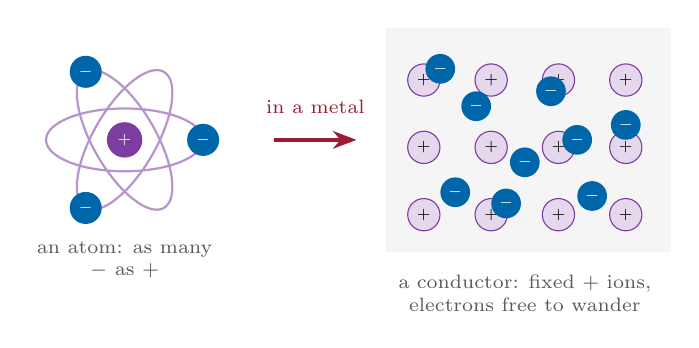
\begin{tikzpicture}[scale=0.95]
  % --- isolated atom
  \draw[ccharge!55, thick] (0,0) ellipse (1.05 and 0.42);
  \begin{scope}[rotate=60]  \draw[ccharge!55, thick] (0,0) ellipse (1.05 and 0.42); \end{scope}
  \begin{scope}[rotate=-60] \draw[ccharge!55, thick] (0,0) ellipse (1.05 and 0.42); \end{scope}
  \node[circle, fill=ccharge, text=white, inner sep=2.2pt, font=\tiny] at (0,0) {$+$};
  \foreach \p in {(1.05,0), (-0.52,0.91), (-0.52,-0.91)}{
    \node[circle, fill=ccur, text=white, inner sep=1.7pt, font=\tiny] at \p {$-$};}
  \node[font=\scriptsize, text=metugray, align=center] at (0,-1.6)
       {an atom: as many\\ $-$ as $+$};
  % --- arrow
  \draw[flowarr] (2.0,0) -- (3.1,0);
  \node[font=\scriptsize, text=metured, align=center, above] at (2.55,0.22) {in a metal};
  % --- lattice
  \begin{scope}[xshift=4.0cm, yshift=-1.0cm]
    \fill[gray!8] (-0.5,-0.5) rectangle (3.3,2.5);
    \foreach \i in {0,1,2,3}{\foreach \j in {0,1,2}{
      \node[circle, draw=ccharge, fill=ccharge!20, inner sep=1.8pt, font=\tiny]
           at (\i*0.9,\j*0.9) {$+$};}}
    \foreach \p in {(0.42,0.3),(1.35,0.7),(2.25,0.25),(0.7,1.45),(1.7,1.65),
                    (2.7,1.2),(0.22,1.95),(2.05,1.0),(1.1,0.15)}{
      \node[circle, fill=ccur, text=white, inner sep=1.4pt, font=\tiny] at \p {$-$};}
    \node[font=\scriptsize, text=metugray, align=center] at (1.35,-1.05)
         {a conductor: fixed $+$ ions,\\ electrons free to wander};
  \end{scope}
\end{tikzpicture}
\end{center}

\vspace{0.4em}

Two facts about charge do all the work in this course:

\begin{enumerate}
  \item \textbf{Charge is conserved.} It is neither created nor destroyed; it only moves.
        When we write Kirchhoff's current law in Lecture~2, we are writing conservation of
        charge.
  \item \textbf{A conductor is already full of charge, and is still neutral.} In a metal,
        roughly one electron per atom breaks loose, leaving a fixed positive ion behind.
        One cubic centimetre of copper contains about $8.5\times10^{22}$ of these ---
        about $13\,600\Cb$ of \emph{mobile} charge --- yet its net charge is essentially
        zero, because every loose electron is matched by the ion it left.
\end{enumerate}

\begin{cautionbox}[What ``free'' does and does not mean]
These are traditionally called \textbf{free electrons}, the term you will meet in your
solid-state and semiconductor courses. But \emph{free} here means free to move
\textbf{within} the metal --- not free to leave it. The electron wanders through the
lattice; it does not escape, and the ion it came from stays put. That is why a piece of
copper can hold $13\,600\Cb$ of movable charge per cubic centimetre and still be neutral.
When the two ideas seem to contradict each other, this word is the trouble; in these notes
the adjective is \textbf{mobile}.
\end{cautionbox}

The second fact is easy to misread. A current in a wire is not charge being \emph{poured
into} the wire: the charge is already there, and a current is that charge
\emph{drifting}. The wire stays neutral while it drifts. This is the first assumption of
the lumped model below, and what makes Kirchhoff's current law true.

\subsection{A pipe that is already full}

The hydraulic picture is the right one, provided you start it correctly: a wire is not an
empty pipe waiting to be filled, but a pipe that is \emph{already full}.

\begin{center}
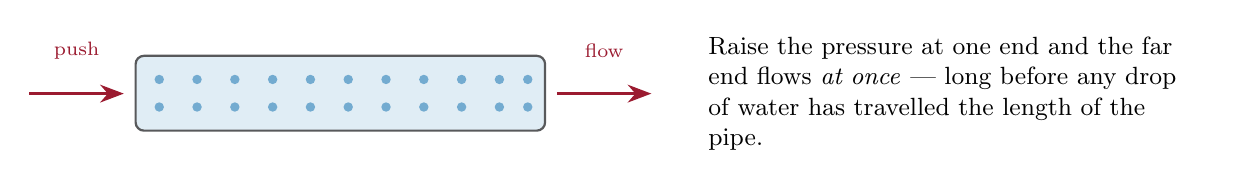
\begin{tikzpicture}[x=1cm,y=1cm]
  \draw[metugray, thick, rounded corners=3pt, fill=ccur!12] (0,0) rectangle (5.2,0.95);
  \foreach \x in {0.30,0.78,1.26,1.74,2.22,2.70,3.18,3.66,4.14,4.62,4.98}{
    \foreach \y in {0.30,0.65}{ \fill[ccur!55] (\x,\y) circle (1.7pt);}}
  \draw[flowarr] (-1.35,0.47) -- (-0.15,0.47);
  \draw[flowarr] (5.35,0.47) -- (6.55,0.47);
  \node[font=\scriptsize, text=metured] at (-0.75,1.02) {push};
  \node[font=\scriptsize, text=metured] at (5.95,1.02) {flow};
  \node[font=\small, anchor=west, text width=6.3cm] at (7.15,0.47)
    {Raise the pressure at one end and the far end flows \emph{at once} --- long before any
     drop of water has travelled the length of the pipe.};
\end{tikzpicture}
\end{center}
\vspace{2pt}

Read across from the picture and most of this lecture is already in it:

\begin{center}
\small
\begin{tabular}{@{}l l@{}}
\toprule
\textbf{pipe already full of water} & \textbf{wire already full of mobile charge}\\
\midrule
pressure difference between the ends & \textbf{voltage} across the element\\
rate of flow past a point & \textbf{current} through it\\
the far end responds immediately & the lamp lights the instant you switch it on\\
water circulates, it is not consumed & charge is not consumed either\\
flow needs a closed loop & so does a circuit\\
\bottomrule
\end{tabular}
\end{center}
\vspace{4pt}

The last two rows head off the two commonest wrong pictures: that a lamp \emph{uses up}
the current passing through it, and that charge can be delivered down a single wire.
Neither survives the full pipe. Whatever flows in at one end flows out at the other, and
it has to come back around.

%==============================================================
\section{Current}

If charge sits still, nothing interesting happens. Circuits are about charge \emph{in
motion}.

\begin{definitionbox}{Electric current}
\textbf{Current} is the time rate of flow of charge through a cross-section:
\[
  \boxed{\;\Icol{i(t)} \;=\; \frac{dq(t)}{dt}\;}
  \qquad\Longleftrightarrow\qquad
  q(t) \;=\; q(t_0) + \int_{t_0}^{t} i(\tau)\,d\tau .
\]
The unit is the \textbf{ampere (A)}, and $1\A = 1\Cb/\s$.
\end{definitionbox}

\begin{center}
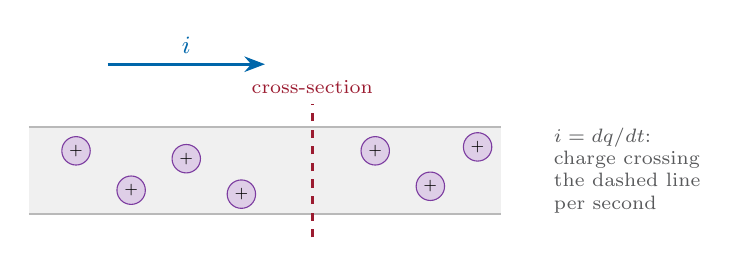
\begin{tikzpicture}[scale=1.0]
  % conductor
  \fill[gray!12] (0,-0.55) rectangle (6,0.55);
  \draw[gray!55, thick] (0,-0.55) -- (6,-0.55);
  \draw[gray!55, thick] (0,0.55) -- (6,0.55);
  % cross-section
  \draw[metured, very thick, dashed] (3.6,-0.85) -- (3.6,0.85);
  \node[metured, font=\scriptsize, above] at (3.6,0.85) {cross-section};
  % charges
  \foreach \x/\y in {0.6/0.25, 1.3/-0.25, 2.0/0.15, 2.7/-0.3, 4.4/0.25, 5.1/-0.2, 5.7/0.3}{
    \node[circle, draw=ccharge, fill=ccharge!25, inner sep=1.3pt, font=\tiny] at (\x,\y) {$+$};
  }
  % current arrow
  \draw[curarr] (1.0,1.35) -- (3.0,1.35) node[midway, above, font=\small] {$\Icol{i}$};
  \node[font=\scriptsize, text=metugray, align=left] at (7.6,0)
       {$i = dq/dt$:\\ charge crossing\\ the dashed line\\ per second};
\end{tikzpicture}
\end{center}

\begin{examplebox}[Example 1.1 --- a coulomb, and the speed of an electron]
\textbf{(a) How much charge does a phone battery hold?} A $4000$ mAh cell:
\[
  Q = 4\A \times 3600\s = 14\,400\Cb ,
  \qquad
  N = \frac{14\,400}{1.602\times10^{-19}} \approx 9\times10^{22}\ \text{electrons}.
\]
The rating is in ampere-hours --- a charge written as a current times a time. Charge comes
in whole electrons, but with $10^{22}$ of them we can treat \Qcol{$q(t)$} as a smooth
function, which is what lets us write $dq/dt$ at all.

\smallskip
\textbf{(b) How fast do the electrons actually move?} Take $1\A$ flowing in an ordinary
$1\ \mathrm{mm^2}$ copper wire. Each electron drifts along the wire at roughly
\[
  0.07\ \mathrm{mm/s} \qquad\text{--- about one metre in four hours.}
\]
Yet the lamp lights the instant you flip the switch. The wire is already full, so you
never wait for an electron to travel from the switch to the lamp: every electron along it
starts moving together, almost the moment you close the circuit.

\smallskip
{\footnotesize (For the curious: the drift speed follows from $v = i/(n e A)$, with
$n \approx 8.5\times10^{28}\ \mathrm{m^{-3}}$ the density of mobile electrons in copper.
Not needed in EE201 --- it is here so the number is not magic.)}
\end{examplebox}

\subsection{Reference direction: the arrow is a choice, not a fact}

A current value is meaningless without an arrow. The arrow declares \emph{which way we
call positive}; the sign of the number then tells us which way the charge actually moves.

\begin{center}
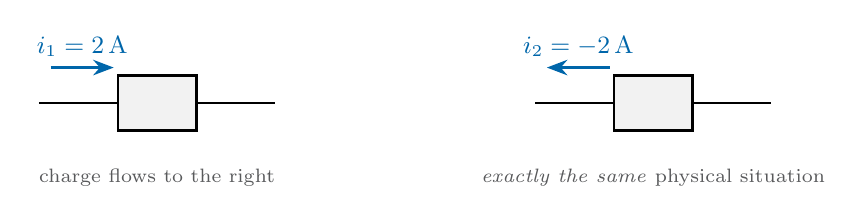
\begin{tikzpicture}
  \begin{scope}
    \draw[thick] (0,0) -- (1,0);
    \draw[thick] (2,0) -- (3,0);
    \draw[thick, fill=gray!10] (1,-0.35) rectangle (2,0.35);
    \draw[curarr] (0.15,0.45) -- (0.95,0.45) node[midway,above,font=\small]{$\Icol{i_1 = 2\A}$};
    \node[font=\scriptsize, text=metugray] at (1.5,-0.95) {charge flows to the right};
  \end{scope}
  \begin{scope}[xshift=6.3cm]
    \draw[thick] (0,0) -- (1,0);
    \draw[thick] (2,0) -- (3,0);
    \draw[thick, fill=gray!10] (1,-0.35) rectangle (2,0.35);
    \draw[curarr] (0.95,0.45) -- (0.15,0.45) node[midway,above,font=\small]{$\Icol{i_2 = -2\A}$};
    \node[font=\scriptsize, text=metugray] at (1.5,-0.95) {\emph{exactly the same} physical situation};
  \end{scope}
\end{tikzpicture}
\end{center}

Both pictures describe the same current. You will often assign arrows before you know the
answer; a negative result is not a mistake, it is the model telling you the charge goes
the other way.

\begin{cautionbox}[Conventional current]
By convention, the current arrow points the way \emph{positive} charge would move. In a
copper wire the carriers are electrons, so they move \emph{against} the arrow.

\smallskip
No equation in this course changes because of it. A current counts only the \emph{net
rate at which charge crosses a section}, and an electron moving left carries as much
charge to the right as a proton moving right. The model never asks what the carriers are
--- and it had better not, since in a semiconductor they are electrons \emph{and} holes,
and in a battery ions.
\end{cautionbox}

\subsection{Notation}

The usual convention: lowercase letters for quantities that may vary with time, uppercase
for constants.
\[
  i(t),\, v(t),\, q(t),\, p(t) \quad\text{(general)}
  \qquad\qquad
  I,\, V,\, Q,\, P \quad\text{(constant, ``DC'')}
\]

\begin{center}
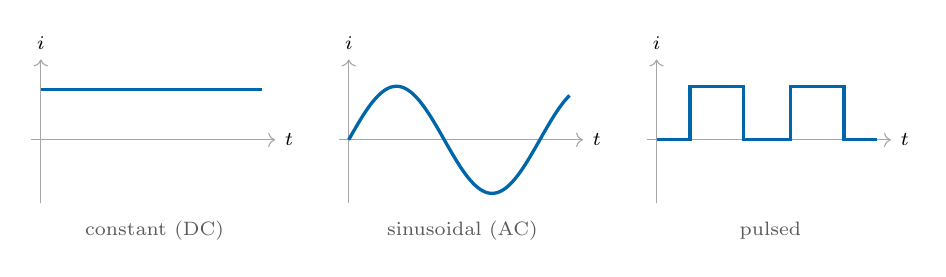
\begin{tikzpicture}[scale=0.85]
 \foreach \dx/\ttl in {0/{constant (DC)}, 4.6/{sinusoidal (AC)}, 9.2/{pulsed}}{
   \begin{scope}[xshift=\dx cm]
     \draw[->,gray!70] (-0.15,0) -- (3.5,0) node[right,font=\scriptsize,black] {$t$};
     \draw[->,gray!70] (0,-0.95) -- (0,1.2) node[above,font=\scriptsize,black] {$i$};
     \node[font=\scriptsize, text=metugray] at (1.7,-1.35) {\ttl};
   \end{scope}
 }
 % DC
 \draw[ccur, very thick] (0,0.75) -- (3.3,0.75);
 % AC
 \begin{scope}[xshift=4.6cm]
   \draw[ccur, very thick, domain=0:3.3, samples=120, smooth]
        plot (\x, {0.8*sin(deg(2.2*\x))});
 \end{scope}
 % pulse
 \begin{scope}[xshift=9.2cm]
   \draw[ccur, very thick] (0,0) -- (0.5,0) -- (0.5,0.8) -- (1.3,0.8) -- (1.3,0)
        -- (2.0,0) -- (2.0,0.8) -- (2.8,0.8) -- (2.8,0) -- (3.3,0);
 \end{scope}
\end{tikzpicture}
\end{center}



\begin{examplebox}[Example 1.2 --- charging a phone]
In the last part of a charge cycle the battery is topped up: the charge \emph{stored in
the battery} approaches its full value as
\[
  q(t) = Q_f\left(1 - e^{-t/\tau}\right),
  \qquad Q_f = 3600\Cb \ (= 1000\ \text{mAh}), \qquad \tau = 20\ \text{min} = 1200\s .
\]
The charging current is the rate at which that charge accumulates:
\[
  i(t) = \frac{dq}{dt} = \frac{Q_f}{\tau}\,e^{-t/\tau}
       = \frac{3600}{1200}\,e^{-t/\tau} = 3\,e^{-t/\tau}\A .
\]
The current starts at $3\A$ and decays: after $20$ minutes it is $3/e \approx 1.1\A$,
after an hour about $0.15\A$. The fuller the battery, the more slowly it fills --- which
is why the last ten per cent takes so long.

\smallskip
With a \emph{constant} current the charge accumulates linearly: $I = 3\A$ flowing for
$8$ hours transports
$Q = I\,\Delta t = 3 \times 8 \times 3600 = 86\,400\Cb$.

\smallskip
\Qcol{Charge} is what accumulates; \Icol{current} is how fast it accumulates. Every
integral--derivative pair in this course has that same flavour.
\end{examplebox}

%==============================================================
\section{Voltage}

Current tells us charge is moving, but not \emph{why} or what the motion costs. Charge
does not wander through a circuit on its own: carrying it through an element exchanges
energy, and voltage is the bookkeeping of that exchange.

Let a small charge $dq$ enter an element at terminal $a$ and leave at $b$, exchanging
energy $dw$ on the way.

\begin{center}
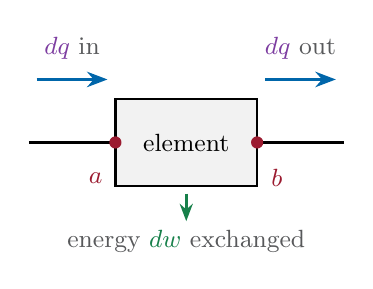
\begin{tikzpicture}[scale=1.0]
  \draw[thick] (0,0) -- (1.1,0); \draw[thick] (2.9,0) -- (4.0,0);
  \draw[thick, fill=gray!10] (1.1,-0.55) rectangle (2.9,0.55);
  \node[font=\small] at (2.0,0) {element};
  \node[font=\small, text=metured] at (0.85,-0.45) {$a$};
  \node[font=\small, text=metured] at (3.15,-0.45) {$b$};
  \fill[metured] (1.1,0) circle (2.2pt); \fill[metured] (2.9,0) circle (2.2pt);
  \draw[curarr] (0.1,0.8) -- (1.0,0.8);
  \node[font=\small, text=metugray] at (0.55,1.2) {\Qcol{$dq$} in};
  \draw[curarr] (3.0,0.8) -- (3.9,0.8);
  \node[font=\small, text=metugray] at (3.45,1.2) {\Qcol{$dq$} out};
  \draw[-{Stealth[length=2.2mm]}, cpow, very thick] (2.0,-0.65) -- (2.0,-1.0);
  \node[font=\small, text=metugray] at (2.0,-1.25) {energy \Pcol{$dw$} exchanged};
\end{tikzpicture}
\end{center}

\begin{definitionbox}{Voltage (potential difference)}
The \textbf{voltage} $\Vcol{v_{ab}}$ between two points $a$ and $b$ is the energy
exchanged \emph{per unit of charge} carried from $a$ to $b$:
\[
  \boxed{\;\Vcol{v_{ab}} \;=\; \frac{\Pcol{dw}}{\Qcol{dq}}\;}
\]
The unit is the \textbf{volt (V)}, and $1\V = 1\J/\Cb$. A positive $v_{ab}$ means the
charge \emph{gives up} energy to the element on its way from $a$ to $b$.
\end{definitionbox}

Four remarks, and they matter more than the formula.

\begin{enumerate}
  \item \textbf{It is a ratio.} Carry twice the charge and twice the energy is exchanged,
        so $v_{ab}$ is the same. Voltage describes the \emph{pair of terminals}, not the
        charge that passed between them.
  \item \textbf{It does not need a current.} A $1.5\V$ battery in a drawer has $1.5\V$
        across its terminals with $i = 0$, just as a closed tap still has pressure behind
        it --- and it still has $1.5\V$ across it while driving $2\A$ through a lamp.
        Voltage is defined, measurable and computable in both cases: it is a readiness to
        exchange energy per unit charge, and says nothing by itself about whether charge
        is flowing. Voltage and current are separate quantities; it takes an
        \emph{element} to relate them, which is what Lecture~3 is about.
  \item \textbf{It is always between two points, and the order matters:}
        $\Vcol{v_{ab}} = -\Vcol{v_{ba}}$. ``The voltage at node $a$'' means nothing until
        a reference point is chosen --- which is why the older name
        \emph{potential difference} is the more honest one.
  \item \textbf{In a lumped circuit it depends only on the two endpoints, not on the
        path between them.} Carry the charge from $a$ to $b$ by any route and the energy
        per unit charge is the same, so ``the voltage between $a$ and $b$'' is a single,
        definite number. This is the second lumped-model assumption in disguise; applied
        around a closed path, it is Kirchhoff's voltage law.
\end{enumerate}

One thing comes for free: with $dq = i\,dt$, the energy exchanged per unit time is
$dw/dt = v\,i$ --- the power, which needs no separate definition.

\subsection{Voltage as an electrical height}

The most useful picture is gravitational. Lifting a mass $m$ through a height $h$ costs
$mgh$; the energy \emph{per unit mass}, $gh$, depends only on the height difference. A
heavier ball gains more energy, but energy per kilogram is the same --- so $gh$, like
voltage, belongs to the two places, not to the object carried between them.

\begin{center}
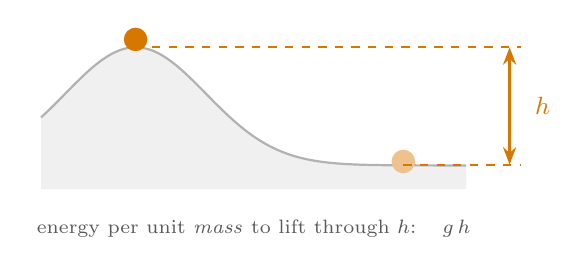
\begin{tikzpicture}[scale=1.0]
  \fill[gray!12] plot[domain=0:5.4, samples=110] (\x, {0.3+1.5*exp(-(\x-1.2)^2/1.6)})
        -- (5.4,0) -- (0,0) -- cycle;
  \draw[gray!60, thick] plot[domain=0:5.4, samples=110]
        (\x, {0.3+1.5*exp(-(\x-1.2)^2/1.6)});
  \node[circle, fill=cvolt, inner sep=3pt] at (1.2,1.9) {};
  \node[circle, fill=cvolt!45, inner sep=3pt] at (4.6,0.35) {};
  \draw[cvolt, thick, dashed] (1.2,1.8) -- (6.1,1.8);
  \draw[cvolt, thick, dashed] (4.6,0.31) -- (6.1,0.31);
  \draw[{Stealth[length=2.2mm]}-{Stealth[length=2.2mm]}, cvolt, very thick]
        (5.95,1.8) -- (5.95,0.31);
  \node[cvolt, font=\small, right] at (6.15,1.05) {$h$};
  \node[font=\scriptsize, text=metugray] at (2.7,-0.5)
       {energy per unit \emph{mass} to lift through $h$: \; $g\,h$};
\end{tikzpicture}
\end{center}

The picture anticipates two later ideas. ``Sea level'' is a choice, and moving it changes
no height difference --- that is ground. And the energy spent climbing a hill does not
depend on the route --- that is remark~4, and Kirchhoff's voltage law.

\subsection{Charge is the amount, voltage is the level}

A trap that catches almost everybody: charge starts to \emph{feel} like energy. It is
not. The way to see why is to separate the \emph{amount} of something from its
\emph{level}.

\begin{center}
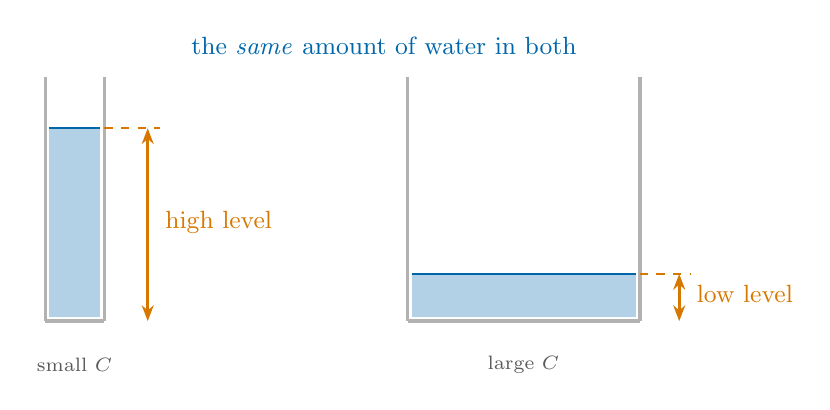
\begin{tikzpicture}[scale=1.0]
  % --- narrow tube
  \draw[gray!60, very thick] (0,0) -- (0,3.1);
  \draw[gray!60, very thick] (0.75,0) -- (0.75,3.1);
  \draw[gray!60, very thick] (0,0) -- (0.75,0);
  \fill[ccur!30] (0.05,0.05) rectangle (0.70,2.45);
  \draw[ccur, thick] (0.05,2.45) -- (0.70,2.45);
  \draw[cvolt, thick, dashed] (0.75,2.45) -- (1.45,2.45);
  \draw[{Stealth[length=2mm]}-{Stealth[length=2mm]}, cvolt, very thick] (1.3,0) -- (1.3,2.45);
  \node[cvolt, font=\small, right] at (1.4,1.25) {high level};
  \node[font=\scriptsize, text=metugray, align=center] at (0.37,-0.55) {small $C$};
  % --- wide tank
  \begin{scope}[xshift=4.6cm]
    \draw[gray!60, very thick] (0,0) -- (0,3.1);
    \draw[gray!60, very thick] (2.95,0) -- (2.95,3.1);
    \draw[gray!60, very thick] (0,0) -- (2.95,0);
    \fill[ccur!30] (0.05,0.05) rectangle (2.90,0.60);
    \draw[ccur, thick] (0.05,0.60) -- (2.90,0.60);
    \draw[cvolt, thick, dashed] (2.95,0.60) -- (3.6,0.60);
    \draw[{Stealth[length=2mm]}-{Stealth[length=2mm]}, cvolt, very thick] (3.45,0) -- (3.45,0.60);
    \node[cvolt, font=\small, right] at (3.55,0.35) {low level};
    \node[font=\scriptsize, text=metugray, align=center] at (1.47,-0.55) {large $C$};
  \end{scope}
  \node[font=\small, text=ccur] at (4.3,3.5) {the \emph{same} amount of water in both};
\end{tikzpicture}
\end{center}

Pour one litre into a narrow tube and the level jumps; pour the same litre into a wide
tank and it barely moves. Same amount, different level, because the containers have
different cross-sections. Electrically, the ``cross-section'' of a pair of conductors is
its \textbf{capacitance} $C$, and the relation is the same:
\[
  q = C\,v .
\]
The \emph{shape of the circuit} plays the part of the shape of the tank: the same charge
moved between a different pair of points gives a different voltage, because the geometry
--- and therefore $C$ --- is different. Capacitance is defined properly in Lecture~4; for
now it is enough that the link between \emph{how much charge} and \emph{what voltage} is a
property of the circuit, not a universal constant.

\begin{ideabox}[Why charge cannot be energy in disguise]
Charge the pair of conductors up to $q$. The energy you had to supply is
\[
  W = \int_0^{q} v\,dq' = \int_0^{q} \frac{q'}{C}\,dq' = \frac{q^2}{2C} = \tfrac{1}{2}Cv^2 .
\]
Two things follow. First, energy grows with the \emph{square} of charge --- if charge
were energy under another name, the relation would be linear. Second, the \emph{first}
coulomb costs almost nothing, because the level is near zero, while the \emph{last} is
expensive, because it must be lifted to the full height. The price of one coulomb
\emph{is} the voltage, and the voltage changes as you fill.
\end{ideabox}

The sharpest statement of the difference is about a complete circuit:

\begin{center}
\begin{minipage}{0.88\textwidth}
\centering\itshape
Around a loop, the charge that leaves the source comes back to it. The energy does not.
\end{minipage}
\end{center}

Charge \emph{circulates}: every coulomb entering a resistor leaves it, none ``used up''.
Energy flows one way --- out of the source, into heat, light or motion, never back. The
copper above makes the same point: one cubic centimetre holds some $13\,600\Cb$ of mobile
charge and stores no energy at all. Charge is everywhere; what carries energy is the
\emph{difference in level}.

%% ---------------------------------------------------------------
%% Kept for Lecture 4, where capacitance is defined properly:
% \begin{ideabox}[For the mechanically minded]
% In the velocity--force analogy of the opening section, mass plays exactly the part of
% capacitance:
% \[
%   p = m\,v \quad\longleftrightarrow\quad q = C\,v ,
%   \qquad
%   \tfrac{1}{2}m v^2 \quad\longleftrightarrow\quad \tfrac{1}{2}C v^2 .
% \]
% Momentum is to velocity what charge is to voltage: the ``amount'' that a given level
% corresponds to, with $m$ or $C$ as the exchange rate. A heavy flywheel is a large
% capacitor --- hard to bring up to speed, and hard to stop.
% \end{ideabox}
%% ---------------------------------------------------------------

\subsection{Reference polarity}

Exactly as for current, we \emph{can} mark a reference polarity with $+$ and $-$ before we
know the answer. The two pictures below describe the same element in the same state.

\begin{center}
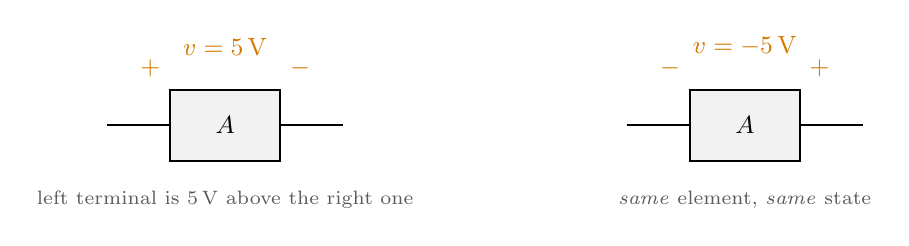
\begin{tikzpicture}
  \begin{scope}
    \draw[thick] (0,0) -- (0.8,0);  \draw[thick] (2.2,0) -- (3.0,0);
    \draw[thick, fill=gray!10] (0.8,-0.45) rectangle (2.2,0.45);
    \node[font=\small] at (1.5,0) {$A$};
    \node[cvolt, font=\small] at (0.55,0.72) {$+$};
    \node[cvolt, font=\small] at (2.45,0.72) {$-$};
    \node[cvolt, font=\small] at (1.5,1.0) {$\Vcol{v = 5\V}$};
    \node[font=\scriptsize, text=metugray] at (1.5,-0.95) {left terminal is $5\V$ above the right one};
  \end{scope}
  \begin{scope}[xshift=6.6cm]
    \draw[thick] (0,0) -- (0.8,0);  \draw[thick] (2.2,0) -- (3.0,0);
    \draw[thick, fill=gray!10] (0.8,-0.45) rectangle (2.2,0.45);
    \node[font=\small] at (1.5,0) {$A$};
    \node[cvolt, font=\small] at (0.55,0.72) {$-$};
    \node[cvolt, font=\small] at (2.45,0.72) {$+$};
    \node[cvolt, font=\small] at (1.5,1.0) {$\Vcol{v = -5\V}$};
    \node[font=\scriptsize, text=metugray] at (1.5,-0.95) {\emph{same} element, \emph{same} state};
  \end{scope}
\end{tikzpicture}
\end{center}

\subsection{The first element: the resistor}

So far we have defined only \emph{variables}: charge, current, voltage. A circuit also
needs \emph{elements}, each imposing a rule between the voltage across it and the current
through it. That rule is the element's \textbf{branch relation}; the whole family arrives
in Lecture~3. One is worth meeting now, because the analogies below need it.

\begin{definitionbox}{The resistor and Ohm's law}
A \textbf{resistor} is a two-terminal element whose voltage and current obey, at every
instant, the algebraic relation
\[
  \boxed{\;\Vcol{v} = R\,\Icol{i}\;}
\]
where $R$ is the \textbf{resistance}, measured in \textbf{ohms} ($\Omega$), with
$1\,\Omega = 1\V/\A$.
\end{definitionbox}

\begin{center}
\begin{circuitikz}[scale=1.0, transform shape]
  \draw (0,0) to[R, l_=$R$, v^=\mbox{\color{cvolt}$v$}, i>_=\mbox{\color{ccur}$i$}] (3.2,0);
\end{circuitikz}
\end{center}

Two features of this relation matter more than the formula.

\begin{itemize}
  \item \textbf{It is algebraic, and has no memory.} The current now is fixed by the
        voltage now --- no derivatives, no integrals, nothing about the past. Such
        elements are called \emph{resistive} (or \emph{static}), and the first four topics
        of the course live entirely among them. Capacitors and inductors, which \emph{do}
        remember, arrive in Lectures~4 and~5 and change the problem completely.
  \item \textbf{The resistance comes from geometry and material.} For a uniform bar of
        length $L$ and cross-section $A$ made of a material of resistivity $\rho$,
        \[
          R = \rho\,\frac{L}{A} .
        \]
        Long and thin means large $R$; short and fat means small $R$ --- exactly the
        behaviour of a pipe carrying water, which is why the next subsection's analogy
        works so well. (Copper has
        $\rho \approx 1.7\times10^{-8}\ \Omega\cdot\mathrm{m}$, which is why we make wires
        out of it and assume they have no resistance at all.)
\end{itemize}

The sign convention that accompanies $v = Ri$, and the reason a resistor can only
\emph{absorb} energy, come once power is defined.

\subsection{The hydraulic analogy}

Most people have better intuition for water than for electrons, and the analogy is close
enough to be useful --- as long as you remember it is an analogy.

\begin{center}
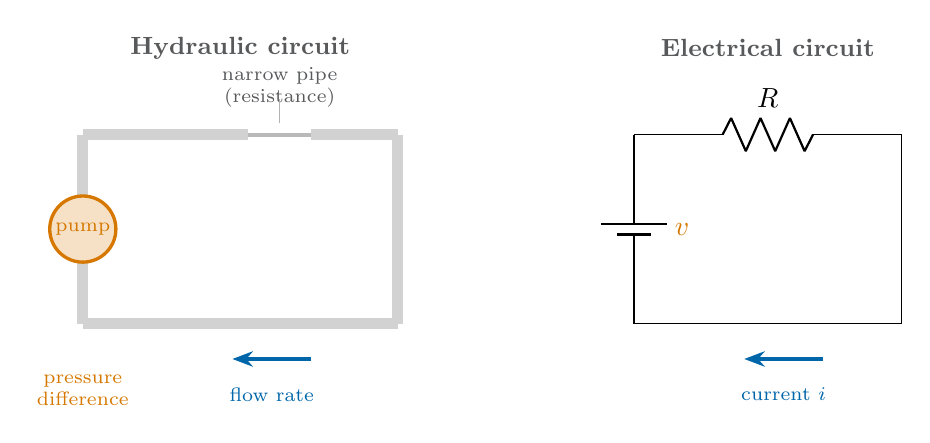
\begin{tikzpicture}[scale=1.0]
%---------------- hydraulic side ----------------
  \node[font=\bfseries\small, text=metugray] at (2.0,3.5) {Hydraulic circuit};
  % pipe loop, with a narrow section on the top edge
  \draw[line width=4pt, gray!35] (0,0) -- (0,2.4);
  \draw[line width=4pt, gray!35] (4,0) -- (4,2.4);
  \draw[line width=4pt, gray!35] (0,0) -- (4,0);
  \draw[line width=4pt, gray!35] (0,2.4) -- (2.1,2.4);
  \draw[line width=1.4pt, gray!55] (2.1,2.4) -- (2.9,2.4);
  \draw[line width=4pt, gray!35] (2.9,2.4) -- (4,2.4);
  \node[font=\scriptsize, text=metugray, align=center] at (2.5,3.0)
       {narrow pipe\\ (resistance)};
  \draw[gray!60] (2.5,2.85) -- (2.5,2.55);
  % pump
  \fill[cvolt!22] (0,1.2) circle (0.42);
  \draw[cvolt, very thick] (0,1.2) circle (0.42);
  \node[font=\scriptsize, text=cvolt] at (0,1.2) {pump};
  \node[font=\scriptsize, text=cvolt, align=center] at (0,-0.85) {pressure\\ difference};
  % flow
  \draw[curarr] (2.9,-0.45) -- (1.9,-0.45);
  \node[font=\scriptsize, text=ccur] at (2.4,-0.9) {flow rate};
%---------------- electrical side ----------------
  \begin{scope}[xshift=7.0cm]
    \node[font=\bfseries\small, text=metugray] at (1.7,3.5) {Electrical circuit};
    \draw (0,0) to[battery1, invert, l_={\color{cvolt}$v$}] (0,2.4);
    \draw (0,2.4) to[R, l={$R$}] (3.4,2.4);
    \draw (3.4,2.4) -- (3.4,0) -- (0,0);
    \draw[curarr] (2.4,-0.45) -- (1.4,-0.45);
    \node[font=\scriptsize, text=ccur] at (1.9,-0.9) {current $i$};
  \end{scope}
\end{tikzpicture}
\end{center}

\begin{center}
\small
\begin{tabular}{@{}l l l@{}}
\toprule
\textbf{Hydraulic} & \textbf{Electrical} & \textbf{Comment}\\
\midrule
pressure (difference)      & \Vcol{voltage $v$}   & the ``across'' quantity: a difference between two points\\
volumetric flow rate       & \Icol{current $i$}   & the ``through'' quantity: needs a direction\\
pipe / tap restriction     & resistance $R$       & opposes flow, dissipates energy\\
pump                       & voltage source       & supplies energy\\
water in the pipes         & \Qcol{charge $q$}    & conserved: it does not disappear\\
\bottomrule
\end{tabular}
\end{center}

%==============================================================
\section{Ground and node voltages}

Since only \emph{differences} of potential have physical meaning, we may declare one point
of the circuit to be zero. That point is the \textbf{reference node}, or \textbf{ground}.

\begin{definitionbox}{Ground (reference node)}
A node chosen, by us, to have potential zero. The ``voltage at node $a$'', written $v_a$,
then means $v_{a,\text{ground}}$, and every two-point voltage follows from
\[
  \boxed{\; v_{ab} = v_a - v_b \;}
\]
\end{definitionbox}

\begin{center}
\begin{circuitikz}[scale=0.95, transform shape]
  \draw (0,0) to[battery1, invert, l_={$12\V$}] (0,2.4);
  \draw (0,2.4) -- (1.2,2.4);
  \draw (1.2,2.4) to[R, l=$R_1$] (3.2,2.4);
  \draw (3.2,2.4) to[R, l=$R_2$, *-*] (3.2,0);
  \draw (3.2,0) -- (0,0);
  \draw (0,0) node[ground]{};
  \node[circle, fill=cvolt, inner sep=1.3pt] at (1.2,2.4) {};
  \node[font=\small, text=cvolt, above left=0pt] at (1.2,2.4) {$a$};
  \node[font=\small, text=cvolt, above right=0pt] at (3.2,2.4) {$b$};
  \node[font=\small, text=metugray, right=2pt] at (3.4,0) {reference: $v = 0$};
  \node[font=\scriptsize, text=metugray, align=left, right=1.1cm] at (4.6,1.6)
    {$v_a = 12\V$\\[2pt] $v_{ab} = v_a - v_b$\\[2pt] $v_{b} = $ voltage across $R_2$};
\end{circuitikz}
\end{center}

Choosing a different ground shifts \emph{every} node voltage by the same constant and
changes \emph{no} two-point voltage, current or power. The choice is convenience: pick the
node the most elements touch, and your equations get shorter.

\begin{ideabox}[Three different things are called ``ground'']
\textbf{Earth ground} is a physical connection to the planet, used for safety.
\textbf{Chassis ground} is the metal enclosure of an instrument. \textbf{Signal ground}
is the analysis reference we have just defined. In EE201 we mean the third one; in the
laboratory, confusing them is how you blow a fuse.
\end{ideabox}

%==============================================================
\section{Power and energy}

\begin{definitionbox}{Power and energy}
\textbf{Power} is the rate at which energy is transferred:
\[
  \boxed{\;\Pcol{p(t)} \;=\; \frac{dw}{dt}
        \;=\; \frac{dw}{dq}\cdot\frac{dq}{dt}
        \;=\; \Vcol{v(t)}\,\Icol{i(t)}\;}
\]
The unit is the \textbf{watt (W)}, $1\W = 1\J/\s$. The energy transferred between $t_0$
and $t$ is
\[
  w(t) = \int_{t_0}^{t} p(\tau)\,d\tau = \int_{t_0}^{t} v(\tau)\,i(\tau)\,d\tau .
\]
\end{definitionbox}

$p = vi$ is not a separate definition: it follows from voltage (energy per charge) and
current (charge per time). That is the whole point of defining them the way we did.

For the one element we have met, Ohm's law gives
\[
  p = vi = i^2 R = \frac{v^2}{R} ,
\]
which for $R > 0$ is never negative, whatever the signs of $v$ and $i$. A resistor can
only \emph{absorb} energy --- it has no way of giving any back --- and that energy leaves
the circuit as heat.

Energy bills are written in kilowatt-hours: $1\ \mathrm{kWh} = 10^3 \times 3600 =
3.6\times10^6\J$.

A units check: a $12\V$ battery supplying a constant $2\A$ for $5$ minutes delivers
\[
  P = VI = 12 \times 2 = 24\W,
  \qquad
  W = P\,\Delta t = 24 \times 300 = 7200\J = 7.2\ \mathrm{kJ}
  = 2\times10^{-3}\ \mathrm{kWh}.
\]

\begin{examplebox}[Example 1.3 --- power that changes in time]
A resistive element carries
\[
  v(t) = 10\cos(\omega t)\V, \qquad i(t) = 2\cos(\omega t)\A ,
  \qquad \omega = 2\pi \cdot 50\ \mathrm{rad/s}.
\]
The instantaneous power is
\[
  p(t) = v(t)\,i(t) = 20\cos^{2}(\omega t) = 10\bigl(1 + \cos 2\omega t\bigr)\W .
\]

\begin{center}
\begin{minipage}[c]{0.52\textwidth}
\centering
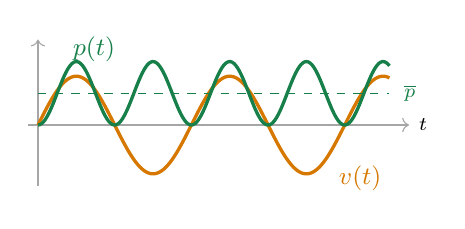
\begin{tikzpicture}[scale=0.62]
  \draw[->,gray!70] (-0.2,0) -- (7.6,0) node[right,font=\scriptsize,black] {$t$};
  \draw[->,gray!70] (0,-1.25) -- (0,1.75);
  \draw[cvolt, very thick, domain=0:7.2, samples=200, smooth]
       plot (\x, {1.0*sin(deg(2*\x))});
  \draw[cpow, very thick, domain=0:7.2, samples=200, smooth]
       plot (\x, {1.3*sin(deg(2*\x))*sin(deg(2*\x))});
  \draw[cpow, dashed] (0,0.65) -- (7.2,0.65);
  \node[cpow, font=\scriptsize, right] at (7.3,0.65) {$\overline{p}$};
  \node[cpow, font=\small] at (1.15,1.55) {$\Pcol{p(t)}$};
  \node[cvolt, font=\small] at (6.6,-1.1) {$\Vcol{v(t)}$};
\end{tikzpicture}
\end{minipage}%
\begin{minipage}[c]{0.46\textwidth}
\small
\begin{itemize}[leftmargin=1.1em]
  \item $p(t) \ge 0$ always: a resistor never returns energy.
  \item The power \emph{oscillates} at twice the frequency of the voltage, about an average
        of $10\W$.
  \item The \emph{peak}, $20\W$, is twice the average. An element must survive the peak;
        how hot it gets is set by the average.
\end{itemize}
\end{minipage}
\end{center}

The energy absorbed over one period $T = 1/50$ s is
\[
  w = \int_{0}^{T} p(t)\,dt = 10\,T + \underbrace{\int_{0}^{T} 10\cos 2\omega t\,dt}_{=\,0}
    = \frac{10}{50} = 0.2\J .
\]
The average power is what a wattmeter shows and what heats the element; the $100$ Hz
oscillation is what makes a cheap transformer hum.
\end{examplebox}

%==============================================================
\section{The passive sign convention}

We have $p = vi$, but $v$ and $i$ each carry a reference that \emph{we} chose. Which sign
of $p$ means ``this element is consuming energy''? A convention settles it.

\begin{definitionbox}{Passive sign convention (PSC)}
Assign the current reference arrow so that it \textbf{enters the terminal marked $+$}.
With that choice,
\[
  \boxed{\;p = vi \;=\; \text{power \emph{absorbed} by the element}\;}
\]
so $p > 0$ means the element absorbs (consumes) energy, and $p < 0$ means it delivers
(supplies) energy to the rest of the circuit.
\end{definitionbox}

\begin{center}
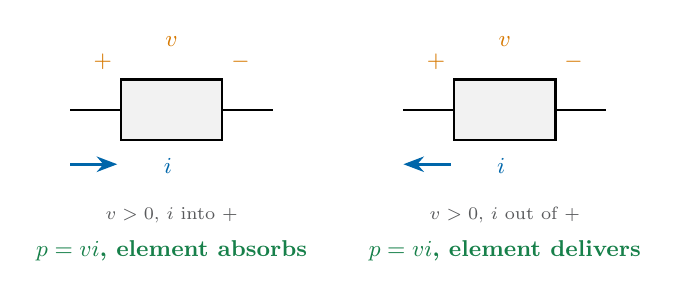
\begin{tikzpicture}[scale=0.92, transform shape]
 \foreach \dx/\sgn/\arr/\lbl/\res in {%
   0/{+}/{right}/{$v>0$, $i$ into $+$}/{absorbs},
   4.6/{+}/{left}/{$v>0$, $i$ out of $+$}/{delivers}}
 {
  \begin{scope}[xshift=\dx cm]
    \draw[thick] (0,0) -- (0.7,0);  \draw[thick] (2.1,0) -- (2.8,0);
    \draw[thick, fill=gray!10] (0.7,-0.42) rectangle (2.1,0.42);
    \node[cvolt, font=\small] at (0.45,0.66) {$+$};
    \node[cvolt, font=\small] at (2.35,0.66) {$-$};
    \node[cvolt, font=\small] at (1.4,0.95) {$\Vcol{v}$};
    \ifnum\pdfstrcmp{\arr}{right}=0
      \draw[curarr] (0.0,-0.75) -- (0.65,-0.75);
    \else
      \draw[curarr] (0.65,-0.75) -- (0.0,-0.75);
    \fi
    \node[ccur, font=\small] at (1.35,-0.78) {$\Icol{i}$};
    \node[font=\scriptsize, text=metugray, align=center] at (1.4,-1.45) {\lbl};
    \node[font=\small\bfseries, text=cpow] at (1.4,-1.95) {$p = vi$, element \res};
  \end{scope}
 }
\end{tikzpicture}
\end{center}

If the picture does \emph{not} satisfy the PSC --- the arrow leaves the $+$ terminal ---
no second formula is needed. Flip one reference, change that variable's sign, and use
$p = vi$:
\[
  p_{\text{absorbed}} = v\,(-i) = -vi .
\]

\subsection{Conservation of power}

Energy is conserved, so in \emph{any} circuit, at \emph{every} instant, the absorbed
powers of all elements sum to zero:
\[
  \boxed{\;\sum_{k=1}^{N} p_k(t) = 0\;}
\]
Elements with $p_k < 0$ (usually sources) supply exactly what those with $p_k > 0$
(usually resistors) consume. This is Tellegen's theorem: if your powers do not cancel,
something is wrong.

\begin{examplebox}[Example 1.4 --- a power balance]
In the circuit below the source drives $2\A$ around the loop and the two resistors drop
$8\V$ and $4\V$.

\begin{center}
\begin{circuitikz}[scale=1.0, transform shape]
  \draw (0,0) to[battery1, invert, l={$12\,$V}] (0,2.6);
  \node[font=\small, text=cvolt] at (-0.33,2.05) {$+$};
  \node[font=\small, text=cvolt] at (-0.33,0.55) {$-$};
  \draw (0,2.6) to[short, i>^={\color{ccur}$2\,$A}] (1.1,2.6);
  \draw (1.1,2.6) to[R, l_={$R_1$}, v^={\color{cvolt}$8\,$V}] (3.9,2.6);
  \draw (3.9,2.6) to[R, l={$R_2$}, v_={\color{cvolt}$4\,$V}] (3.9,0);
  \draw (3.9,0) -- (0,0);
\end{circuitikz}
\end{center}

With the PSC applied to each element:
\[
  p_{R_1} = 8 \times 2 = +16\W, \qquad
  p_{R_2} = 4 \times 2 = +8\W, \qquad
  p_{\text{source}} = 12 \times (-2) = -24\W .
\]
The source current leaves its $+$ terminal, hence the $-2\A$; the sum is
$16 + 8 - 24 = 0$, as it must be. The source \emph{delivers} $24\W$ and the resistors
\emph{absorb} it.
\end{examplebox}

%==============================================================
\section{Electric circuits and the lumped model}

\begin{definitionbox}{Electric circuit}
An \textbf{electric circuit} is an interconnection of electrical elements through which
charge can flow along closed paths.
\end{definitionbox}

Everything we do in EE201 rests on one further modelling assumption, worth stating
precisely rather than assuming silently.

\begin{definitionbox}{The lumped circuit model}
A circuit is \textbf{lumped} when three things may be assumed.

\medskip
\textbf{(a) Nothing piles up.} At every instant, the current leaving an element equals the
current entering it.

\textbf{(b) Nothing leaks out.} No changing \emph{magnetic} field passes through the loops
formed by your wiring, and no charge on one element pulls on the charge in another across
the space between them. The fields belong to the elements, not to the space between them.

\textbf{(c) Nothing is late.} A signal of frequency $f$ travelling at the speed of light
$c$ advances a distance $\lambda = c/f$ in one period; $\lambda$ is its
\textbf{wavelength}. The circuit, of size $d$, must be much smaller than that:
\[
   \boxed{\; d \;\ll\; \lambda = \frac{c}{f} \;},
   \qquad c \approx 3\times10^8\ \mathrm{m/s}.
\]
\end{definitionbox}

Read (c) in terms of times if you prefer: crossing the circuit takes $d/c$, the signal
changes in $1/f$, and we assume the first is negligible next to the second. Either way, a
change at one point reaches everywhere else before anything else has had time to happen.

When the three hold, a circuit is described by \emph{ordinary} differential equations in
time. When they do not, the same physics needs Maxwell's equations and partial
differential equations in space and time --- what the electromagnetic field theory courses
are for.

\begin{center}
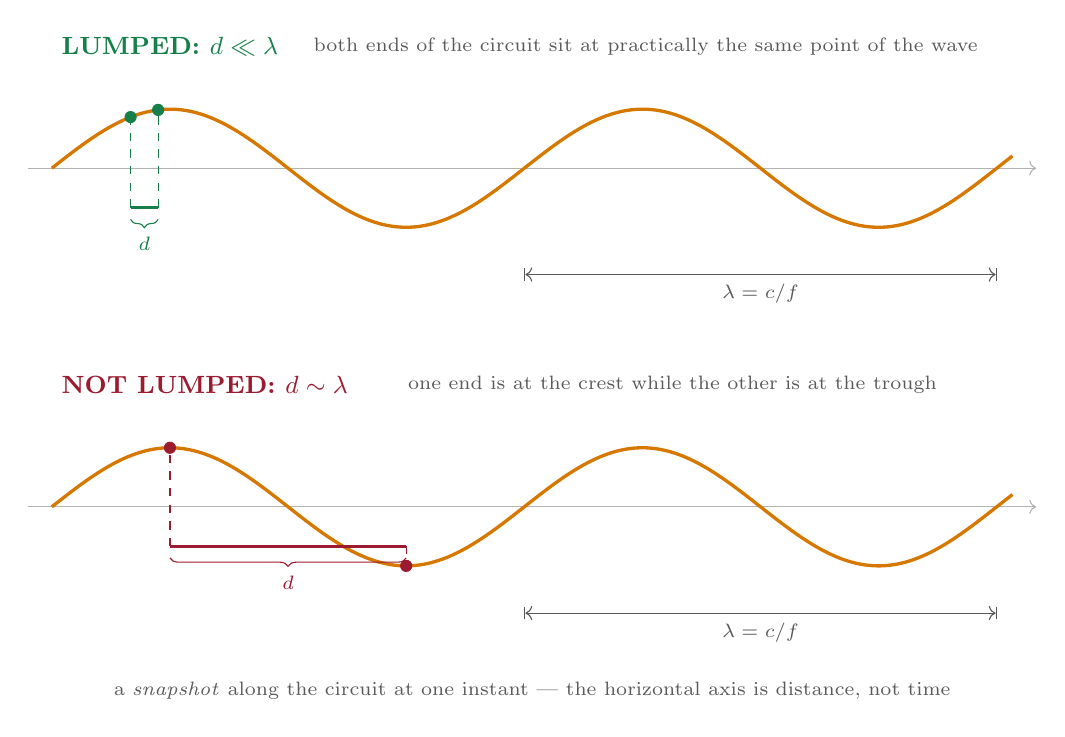
\begin{tikzpicture}[x=1cm,y=1cm]
  % ---- panel (a): lumped
  \begin{scope}
    \node[font=\small\bfseries,text=cpow,anchor=west] at (0,1.55) {LUMPED: $d \ll \lambda$};
    \node[font=\scriptsize,text=metugray,anchor=west] at (3.2,1.55)
         {both ends of the circuit sit at practically the same point of the wave};
    \draw[->,gray!60] (-0.3,0) -- (12.5,0);
    \draw[cvolt, very thick, domain=0:12.2, samples=300, smooth] plot (\x, {0.75*sin(60*\x)});
    \draw[metugray,|<->|] (6,-1.35) -- (12,-1.35) node[midway,below,font=\scriptsize] {$\lambda = c/f$};
    \fill[cpow] (1.0,{0.75*sin(60*1.0)}) circle (2.2pt);
    \fill[cpow] (1.35,{0.75*sin(60*1.35)}) circle (2.2pt);
    \draw[cpow,dashed,thin] (1.0,-0.5) -- (1.0,{0.75*sin(60*1.0)});
    \draw[cpow,dashed,thin] (1.35,-0.5) -- (1.35,{0.75*sin(60*1.35)});
    \draw[cpow, very thick] (1.0,-0.5) -- (1.35,-0.5);
    \draw[cpow, decorate, decoration={brace,mirror,amplitude=3pt}] (1.0,-0.65) -- (1.35,-0.65)
          node[midway,below=3pt,font=\scriptsize] {$d$};
  \end{scope}
  % ---- panel (b): not lumped
  \begin{scope}[yshift=-4.3cm]
    \node[font=\small\bfseries,text=metured,anchor=west] at (0,1.55) {NOT LUMPED: $d \sim \lambda$};
    \node[font=\scriptsize,text=metugray,anchor=west] at (4.4,1.55)
         {one end is at the crest while the other is at the trough};
    \draw[->,gray!60] (-0.3,0) -- (12.5,0);
    \draw[cvolt, very thick, domain=0:12.2, samples=300, smooth] plot (\x, {0.75*sin(60*\x)});
    \draw[metugray,|<->|] (6,-1.35) -- (12,-1.35) node[midway,below,font=\scriptsize] {$\lambda = c/f$};
    \fill[metured] (1.5,0.75) circle (2.2pt);
    \fill[metured] (4.5,-0.75) circle (2.2pt);
    \draw[metured,dashed,thin] (1.5,-0.5) -- (1.5,0.75);
    \draw[metured,dashed,thin] (4.5,-0.5) -- (4.5,-0.75);
    \draw[metured, very thick] (1.5,-0.5) -- (4.5,-0.5);
    \draw[metured, decorate, decoration={brace,mirror,amplitude=3pt}] (1.5,-0.65) -- (4.5,-0.65)
          node[midway,below=3pt,font=\scriptsize] {$d$};
  \end{scope}
  \node[font=\scriptsize,text=metugray,anchor=north] at (6.1,-6.4)
       {a \emph{snapshot} along the circuit at one instant --- the horizontal axis is distance, not time};
\end{tikzpicture}
\end{center}

The picture above is the one to keep. It shows the signal \emph{frozen in space}: the
horizontal axis runs along the circuit, and the curve is the signal's value at each place
at one instant. If the circuit occupies a tiny fraction of a wavelength, every point reads
the same number and we may speak of ``the'' voltage of a node. If it occupies an
appreciable fraction, different parts hold different values at the same moment, and a
single node voltage no longer exists.

Each of the three, translated:

\begin{itemize}
  \item \textbf{(a) does not forbid charge from moving \emph{inside} an element.} A
        capacitor is the obvious case: it puts $+q$ on one plate and $-q$ on the other, so
        charge does separate inside it. (a) says the element as a \emph{whole} never gains
        or loses charge --- the same current $i = dq/dt$ that enters one terminal leaves
        the other. A wire, likewise, is a pipe and not a bucket. Without this, ``the
        current through an element'' would not be well defined, and Kirchhoff's current
        law would be false.
  \item \textbf{(b) says the loops in your diagram are not antennas and not
        transformers.} You drew a rectangle of wire; a changing \emph{magnetic} field
        through it would induce a voltage, and the voltage between two nodes would depend
        on how you routed the wire. Assumption (b) rules that out, which makes ``the
        voltage between $a$ and $b$'' independent of the path --- and Kirchhoff's voltage
        law true.
  \item \textbf{(c) says everything happens everywhere at once.} A signal crosses a
        $30$ cm board in about a nanosecond, while a $50$ Hz mains waveform takes
        milliseconds to change appreciably --- a factor of a million. That delay is not
        worth modelling, so one time variable $t$ serves the whole circuit, with no
        dependence on position.
\end{itemize}

\begin{center}
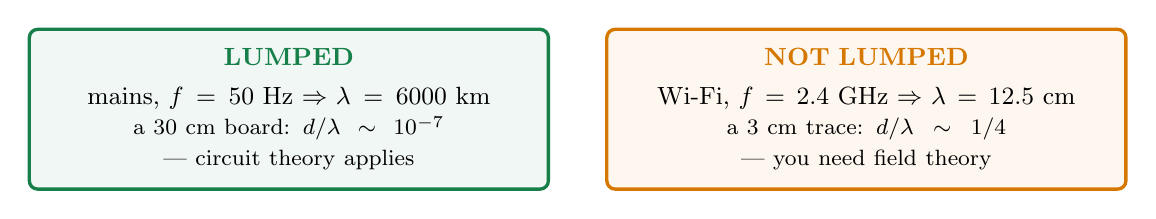
\begin{tikzpicture}[node distance=0.7cm]
  \node[draw=cpow, very thick, fill=cpow!6, rounded corners=3pt,
        text width=6.1cm, align=center, inner sep=7pt, font=\small] (L)
       {\textbf{\textcolor{cpow}{LUMPED}}\\[3pt]
        mains, $f = 50$ Hz $\Rightarrow$ $\lambda = 6000$ km\\
        {\footnotesize a $30$ cm board: $d/\lambda \sim 10^{-7}$ --- circuit theory applies}};
  \node[draw=cvolt, very thick, fill=cvolt!6, rounded corners=3pt,
        text width=6.1cm, align=center, inner sep=7pt, font=\small, right=of L] (R)
       {\textbf{\textcolor{cvolt}{NOT LUMPED}}\\[3pt]
        Wi-Fi, $f = 2.4$ GHz $\Rightarrow$ $\lambda = 12.5$ cm\\
        {\footnotesize a $3$ cm trace: $d/\lambda \sim 1/4$ --- you need field theory}};
\end{tikzpicture}
\end{center}

The same hardware can be lumped for one signal and distributed for another. A mobile phone
motherboard is a lumped circuit for its battery and a transmission-line problem for its
antenna. The model is chosen by the question, not by the object.

%==============================================================
\section{Terminals, nodes, branches}

The last piece of vocabulary describes how elements are connected --- the topology.

\begin{definitionbox}{Terminal, node, branch, loop}
\begin{itemize}[leftmargin=1.3em]
  \item A \textbf{terminal} is a point at which an element can be connected to others. A
        resistor, capacitor or inductor has two terminals; a transistor has three; an
        op-amp has five or more.
  \item A \textbf{node} is a point of connection between two or more elements. Everything
        joined by ideal (zero-resistance) wire is \emph{one and the same node}, however
        long the wire is drawn.
  \item A \textbf{branch} is a single element between two nodes.
  \item A \textbf{loop} is a closed path through the circuit that does not pass through
        any node more than once.
\end{itemize}
\end{definitionbox}

\begin{center}
\begin{circuitikz}[scale=0.95, transform shape]
  \draw (0,0) to[battery1, invert, l_={$V_s$}] (0,2.4);
  \draw (0,2.4) -- (1.0,2.4);
  \draw (1.0,2.4) to[R, l=$R_1$] (3.4,2.4);
  \draw (3.4,2.4) to[R, l=$R_2$] (3.4,0);
  \draw (3.4,2.4) -- (5.0,2.4);
  \draw (5.0,2.4) to[R, l=$R_3$] (5.0,0);
  \draw (5.0,0) -- (0,0);
  \draw (0,0) node[ground]{};
  % node dots
  \foreach \p in {(1.0,2.4),(3.4,2.4),(5.0,2.4)}{\fill[metured] \p circle (2.2pt);}
  \fill[metured] (0,0) circle (2.2pt);
  \node[font=\small, text=metured, above] at (0.7,2.5) {$n_1$};
  \node[font=\small, text=metured, above] at (3.4,2.55) {$n_2$};
  \node[font=\small, text=metured, below] at (1.7,-0.1) {$n_3$ (ground)};
\end{circuitikz}
\end{center}

In the figure, $n_2$ is a single node even though three elements meet there through a
stretch of wire; the wire itself is not a branch. Counting: $3$ nodes, $4$ branches
($V_s$, $R_1$, $R_2$, $R_3$) and $2$ independent loops, consistent with the relation you
will meet in Lecture~2,
\[
  \#\text{branches} = \#\text{loops} + \#\text{nodes} - 1
  \qquad\Longrightarrow\qquad 4 = 2 + 3 - 1 .
\]

\begin{examplebox}[Example 1.5 --- the same circuit, drawn twice]
The two drawings below look different but are the \emph{same} circuit: in both, $R_1$ and
$R_2$ share both terminals, and that pair is in series with $R_3$ and the source.

\begin{center}
\begin{circuitikz}[scale=0.78, transform shape]
  \draw (0,0) to[battery1, invert, l={$V_s$}] (0,2.8);
  \draw (0,2.8) -- (1.6,2.8);
  \draw (1.6,2.8) to[R, l_={$R_1$}] (1.6,1.0);
  \draw (3.6,2.8) to[R, l={$R_2$}] (3.6,1.0);
  \draw (1.6,2.8) -- (3.6,2.8);
  \draw (1.6,1.0) -- (3.6,1.0);
  \draw (1.6,1.0) -- (1.6,0.5);
  \draw (3.6,1.0) -- (3.6,0.5);
  \draw (1.6,0.5) -- (5.8,0.5);
  \draw (5.8,0.5) to[R, l={$R_3$}] (5.8,2.8);
  \draw (5.8,2.8) -- (6.9,2.8) -- (6.9,0) -- (0,0);
  \draw (0,0) node[ground]{};
  \foreach \pt in {(1.6,2.8),(1.6,0.5)}{\fill[metured] \pt circle (2.4pt);}
  \node[font=\scriptsize, text=metugray] at (3.4,-0.6) {drawing (a)};
\end{circuitikz}
\hspace{0.7cm}
\begin{circuitikz}[scale=0.78, transform shape]
  \draw (0,0) to[battery1, invert, l={$V_s$}] (0,2.6);
  \draw (0,2.6) -- (1.2,2.6);
  \draw (1.2,2.6) to[R, l_={$R_1$}] (3.0,2.6);
  \draw (1.2,1.5) to[R, l_={$R_2$}] (3.0,1.5);
  \draw (1.2,2.6) -- (1.2,1.5);
  \draw (3.0,2.6) -- (3.0,1.5);
  \draw (3.0,2.05) -- (4.0,2.05);
  \draw (4.0,2.05) to[R, l={$R_3$}] (4.0,0);
  \draw (4.0,0) -- (0,0);
  \draw (0,0) node[ground]{};
  \foreach \pt in {(1.2,2.6),(3.0,2.6)}{\fill[metured] \pt circle (2.2pt);}
  \node[font=\scriptsize, text=metugray] at (2.0,-0.65) {drawing (b)};
\end{circuitikz}
\end{center}

Drawing (b) makes it obvious that $R_1$ and $R_2$ are in parallel; drawing (a) hides it
behind a detour of wire. Only the placement of the symbols changed --- and that is the
only skill being tested when a problem looks impossible at first sight.
\end{examplebox}

\begin{cautionbox}[Drawing is not topology]
Two circuits that look completely different on paper can be the same circuit. What
matters is which terminals share a node, not where you placed the symbols. So when a
problem looks unfamiliar, redraw it: put every element on a given node so that it visibly
touches the \emph{same point or the same line}, and straighten the detours of wire. Series
and parallel connections usually become obvious, and half the difficulty goes with them.
\end{cautionbox}

%==============================================================
\section*{Summary}
\addcontentsline{toc}{section}{Summary}

\begin{center}
\small
\begin{tabular}{@{}l l l l@{}}
\toprule
\textbf{Quantity} & \textbf{Symbol} & \textbf{Defining relation} & \textbf{Unit}\\
\midrule
charge  & \Qcol{$q$} & --- & coulomb, C\\
current & \Icol{$i$} & $i = dq/dt$ & ampere, A $=$ C/s\\
voltage & \Vcol{$v$} & $v = dw/dq$ & volt, V $=$ J/C\\
power   & \Pcol{$p$} & $p = dw/dt = vi$ & watt, W $=$ J/s\\
energy  & \Pcol{$w$} & $w = \int p\,dt$ & joule, J\\
\bottomrule
\end{tabular}
\end{center}

\begin{itemize}
  \item Current needs a \textbf{reference arrow}; voltage needs a \textbf{reference
        polarity}. Both are choices. A negative answer is information, not an error.
  \item With the \textbf{passive sign convention} (current into the $+$ terminal),
        $p = vi$ is the absorbed power, and $\sum_k p_k = 0$ over the whole circuit.
  \item Voltage is an \textbf{across} quantity, current is a \textbf{through} quantity;
        ground is the node we \emph{choose} to call zero.
  \item The \textbf{lumped} assumption ($d \ll \lambda$, no charge accumulation, no stray
        flux) is what lets us use ordinary differential equations for the rest of the
        course.
\end{itemize}

\subsection*{Next lecture}
Interconnection laws --- Kirchhoff's current and voltage laws --- and the branch relations
of the basic elements. Everything from Lecture~1 is used there without further comment.

\subsection*{Reading}
\begin{itemize}
  \item Alexander \& Sadiku, \emph{Fundamentals of Electric Circuits}, Chapter~1.
  \item Chua, Desoer \& Kuh, \emph{Linear and Nonlinear Circuits}, Chapter~1.
  \item Lecture notes and videos of Prof.\ Emre Tuna,
        \href{https://users.metu.edu.tr/etuna/ee201/}{\texttt{users.metu.edu.tr/etuna/ee201}}.
\end{itemize}

\end{document}
